% !TEX root = ../document.tex
% !TeX spellcheck = pt_BR

\section{O ciclo cardíaco e alterações}

\begin{frame}{O ciclo cardíaco}
    \begin{center}
        \includegraphics[scale=0.25]{figures/cardiac-cycle.pdf}
    \end{center}
    \tiny Extraído de:\\
    \url{http://en.wikipedia.org/wiki/File:SinusRhythmLabels.svg}
\end{frame}

\begin{frame}{Efeitos da isquemia}
    \begin{columns}[t]
        \column{0.5\textwidth}
            Depressão do segmento ST:\\
            \center
            \begin{tikzpicture}
                \node[anchor=south west,inner sep=0] at (0,0) {\includegraphics[width=\textwidth]{figures/st-dep.pdf}};
                \draw[red,thick] (3.4,0.9) circle [x radius=24pt, y radius=15pt];
            \end{tikzpicture}
        \column{0.5\textwidth}
            Elevação do segmento ST:\\
            \center
            \begin{tikzpicture}
                \node[anchor=south west,inner sep=0] at (0,0) {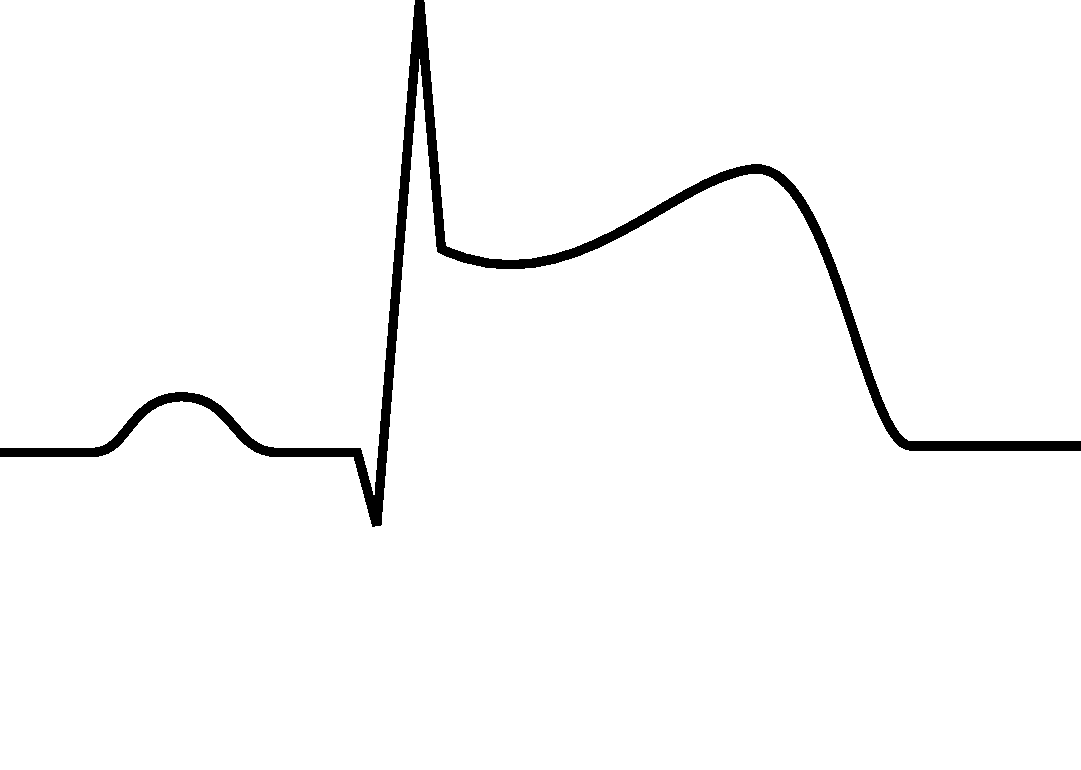
\includegraphics[width=\textwidth]{figures/st-elev.pdf}};
                \draw[red,thick] (3.2,3.0) circle [x radius=24pt, y radius=15pt];
            \end{tikzpicture}
    \end{columns}
\end{frame}

\begin{frame}{Efeitos da isquemia}
    \begin{columns}[t]
        \column{0.5\textwidth}
            Onda T normal:\\
            \center
            \begin{tikzpicture}
                \node[anchor=south west,inner sep=0] at (0,0) {\includegraphics[width=\textwidth]{figures/t-normal.pdf}};
                %\draw[red,thick] (4.5,1.0) circle [x radius=25pt, y radius=25pt];
            \end{tikzpicture}
        \column{0.5\textwidth}
            Onda T invertida:\\
            \center
            \begin{tikzpicture}
                \node[anchor=south west,inner sep=0] at (0,0) {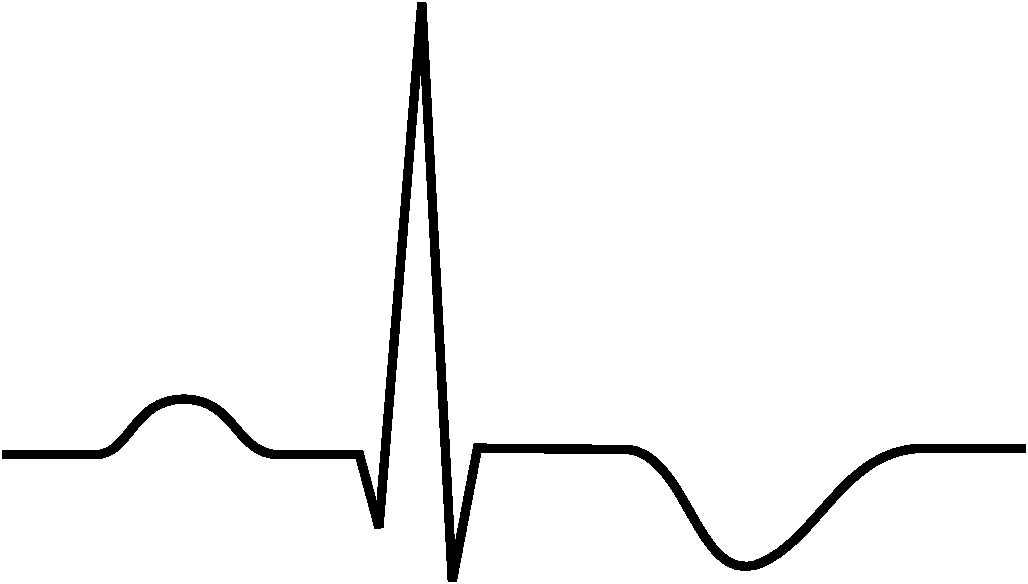
\includegraphics[width=\textwidth]{figures/t-inverted.pdf}};
                \draw[red,thick] (4.4,0.6) circle [x radius=25pt, y radius=25pt];
            \end{tikzpicture}
    \end{columns}
\end{frame}
